\documentclass[14pt]{beamer}

% beamer definieert 'definition' al, maar dan engels :(
% fix van:
% http://tex.stackexchange.com/questions/38392/how-to-rename-theorem-or-lemma-in-beamer-to-another-language
\usepackage[dutch]{babel}
\uselanguage{dutch}
\languagepath{dutch}
\deftranslation[to=dutch]{Definition}{Definitie}
\deftranslation[to=dutch]{Example}{Voorbeeld}

\definecolor{todocolor}{rgb}{1, 0.3, 0.2}
\newcommand{\td}[1]{\colorbox{todocolor}{*\footnote{TODO: #1}}}
\newcommand{\from}{\leftarrow}

\usepackage{array}

\usepackage{graphicx}
\usepackage{float}
\usepackage{amssymb}
\usepackage{color}
\usepackage{listings}

\newcommand{\id}{\text{id}}
\newcommand{\N}{\mathbb{N}}
\newcommand{\Z}{\mathbb{Z}}
\newcommand{\R}{\mathbb{R}}
\newcommand{\cat}[1]{\mathbf{#1}}
\newcommand{\Ch}[1]{\mathbf{Ch}(#1)}
\newcommand{\Hom}[3]{\mathbf{Hom}_{#1}(#2, #3)}

\newcommand{\iso}{\cong}
\newcommand{\tot}[1]{\xrightarrow{\,\,{#1}\,\,}}
\newcommand{\eps}{\varepsilon}
\newcommand{\I}{\,\mid\,}
\newcommand{\then}{\Rightarrow}
\newcommand{\inject}{\hookrightarrow}
\newcommand{\del}{\partial}
\newcommand{\nsubgrp}{\trianglelefteq}

% relative to the one who includes us :(
\graphicspath{ {../images/} }

\newcommand{\todo}[1]{
	\addcontentsline{tdo}{todo}{\protect{#1}}
	$\ast$ \marginpar{\tiny $\ast$ #1}
}
\makeatletter
	\newcommand \listoftodos{\section*{Todo list} \@starttoc{tdo}}
	\newcommand\l@todo[2]{
		\par\noindent \textit{#2}, \parbox{10cm}{#1}\par
	}
\makeatother

\graphicspath{ {../presentation2/images/} {../thesis/images/} }

\title{De Dold-Kan correspondentie
	\huge $$ \Ch{\Ab} \simeq \sAb $$}
\author{Joshua Moerman}
\institute[Radboud Universiteit Nijmegen]{Begeleid door Moritz Groth}
\date{}

\begin{document}


\begin{frame}
	\titlepage
\end{frame}

\begin{frame}{Categorie\"en}
	Een \emph{categorie} $\cat{C}$ bestaat uit
	
	\begin{center}
		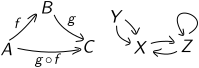
\includegraphics{cat_th}
	\end{center}

	met \emph{compositie} $-\circ-$, zodat
	\begin{itemize}
		\item er is een \emph{identiteit} $\id_c: C \to C$ en
		\item compositie is associatief.
	\end{itemize}
\end{frame}

\begin{frame}
	\frametitle{Voorbeelden}
	\begin{itemize}
		\item[$\Set$]
			objecten: verzamelingen \\
			pijlen: functies
		\item[$\Ab$]
			objecten: abelse groepen \\
			pijlen: groupshomomorfismes
		\item[$\cat{\underline{4}}$] 
		\tikz[baseline=-0.5ex]{
			\matrix (m) [matrix of math nodes, row sep=2em, column sep=2em, ampersand replacement=\&]{
				\ast_1 \& \ast_2 \\
				\ast_3 \& \ast_4 \\
			};
			\path[->] (m-1-1) edge node[font=\small, auto] {$ a $} (m-1-2);
			\path[->] (m-1-1) edge node[font=\small, auto] {$ f $} (m-2-1);
			\path[->] (m-1-2) edge node[font=\small, auto] {$ b $} (m-2-2);
			\path[->] (m-2-1) edge node[font=\small, auto] {$ g $} (m-2-2);
		} \hspace{1cm} met $ba = gf$.
	\end{itemize}
\end{frame}

\begin{frame}
	\frametitle{Functors}
	Een \emph{functor} $F: \cat{C} \to \cat{D}$ is een functie op objecten \'en pijlen.

	\begin{center}
		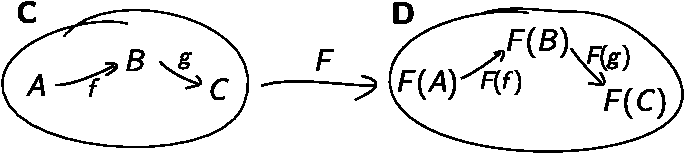
\includegraphics[scale=0.9]{cat_functor}
	\end{center}

	Zodat
	\begin{itemize}
		\item $F(\id_C) = \id_{F(C)}$ en
		\item $F(g \circ f) = F(g) \circ F(f)$.
	\end{itemize}
\end{frame}

\begin{frame}
	\frametitle{Voorbeeld functor}

	Voor een verzameling $V$ definieer
	$$ \Z[V] = \{ \phi: V \to \Z \I \phi(v) \neq 0 \text{ voor eindig veel } v \}. $$

	\bigskip
	Voor een functie $f: V \to W$ definieer
	\begin{gather*}
		\Z[f]: \Z[V] \to \Z[W] \\
		\Z[f](\phi) = \sum_v \phi(v) \chi_{\{f(v)\}}.
	\end{gather*}

	\bigskip
	Dit is een functor: $\Z[-]: \Set \to \Ab$.
\end{frame}

\begin{frame}
	\frametitle{Voorbeeld functor}

	Definieer $F: \cat{\underline{4}} \to \Ab$ als volgt:
	$$ F(\ast_1) = F(\ast_2) = F(\ast_3) = F(\ast_4) = \Z $$
	en op pijlen:
	\begin{align*}
		F(f)(n) = 4n & & F(g)(n) = 3n \\
		F(a)(n) = 6n & & F(b)(n) = 2n.
	\end{align*}

	\begin{columns}
		\begin{column}{0.5\textwidth}
		\tikz[baseline=-0.5ex]{
			\matrix (m) [matrix of math nodes, row sep=2em, column sep=2em, ampersand replacement=\&]{
				\Z \& \Z \\
				\Z \& \Z \\
			};
			\path[->] (m-1-1) edge node[font=\small, auto] {$ \times 6 $} (m-1-2);
			\path[->] (m-1-1) edge node[font=\small, auto] {$ \times 4 $} (m-2-1);
			\path[->] (m-1-2) edge node[font=\small, auto] {$ \times 2 $} (m-2-2);
			\path[->] (m-2-1) edge node[font=\small, auto] {$ \times 3 $} (m-2-2);
		}
		\end{column}
		\begin{column}{0.5\textwidth}
		Compositie is behouden, want het diagram commuteert.
		\end{column}
	\end{columns}
\end{frame}

\begin{frame}
	\frametitle{Samenvattend}
	\begin{itemize}
		\item Categorie $\stackrel{D}{=}$ objecten + pijlen.
		\item Functor $\stackrel{D}{=}$ pijl tussen categorie\"en.
	\end{itemize}

	\begin{itemize}
		\item Functor $\sim$ Constructies.
		\item Functor $\sim$ Diagrammen.
	\end{itemize}

	\bigskip\pause
	$F$ is \emph{contravariant} (notatie $F: \cat{C}^{op} \to \cat{D}$) als
	\begin{columns}
		\begin{column}{0.7\textwidth}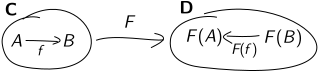
\includegraphics[scale=0.8]{cat_contrafunctor}\end{column}
		\begin{column}{0.3\textwidth}\small $F(g \circ f) = F(g) \circ F(f)$.\end{column}
	\end{columns}
\end{frame}

\begin{frame}
	\frametitle{Belangrijke categorie in mijn scriptie}

	\begin{itemize} \item[$\DELTA$]
			objecten: $[n] = \{0, \ldots, n\}$, $n\in\N$ \\
			pijlen: monotoon stijgende functies.
	\end{itemize}

	\bigskip
	\only<1>{\begin{example}
		Voor elke $n \in \N$ zijn er pijlen
	\end{example}}
	\only<2->{\begin{lemma}
		Elke pijl in $\DELTA$ is een compositie van
	\end{lemma}}
	\begin{itemize}
		\item $\delta_i: [n] \mono [n+1]$ slaat $i$ over \hfill ($0 \leq i \leq n$)
		\item $\sigma_i: [n+1] \epi [n]$ bereik $i$ twee keer \hfill ($0 \leq i < n$)
	\end{itemize}

	\visible<3>{
		Dus $\DELTA = \vcenter{\hbox{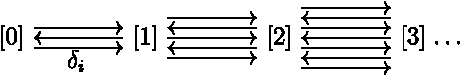
\includegraphics{delta_cat}}}$
	}
\end{frame}

\begin{frame}
	\frametitle{Belangrijke categorie in mijn scriptie}

	$\DELTA = \vcenter{\hbox{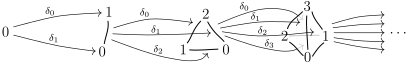
\includegraphics[scale=0.8]{delta_cat_geom}}}$

	\pause\bigskip
	\begin{lemma}
		De \emph{cosimpliciale vergelijkingen} gelden:
		\small
		\begin{align*}
			\delta_j\delta_i &= \delta_i\delta_{j-1},  \hspace{1.5cm} \textnormal{ if } i < j,\\
			\sigma_j\delta_i &= \delta_i\sigma_{j-1},  \hspace{1.5cm} \textnormal{ if } i < j,\\
			\sigma_j\delta_j &= \sigma_j\delta_{j+1} = \id,\\
			\sigma_j\delta_i &= \delta_{i-1}\sigma_j,  \hspace{1.5cm} \textnormal{ if } i > j+1,\\
			\sigma_j\sigma_i &= \sigma_i\sigma_{j+1},  \hspace{1.5cm} \textnormal{ if } i \leq j.
		\end{align*}
	\end{lemma}
\end{frame}

\begin{frame}
\begin{center}
	\Large \visible<2->{$A:$} $\DELTA^{op} \to \Ab$ \visible<2->{\hspace{1cm}}

	\bigskip
	\visible<2->{
	$$ A := 
	\begin{tikzpicture}[baseline=-0.5ex]
	\matrix (m) [matrix of math nodes, ampersand replacement=\&, row sep=2em, column sep=2em] { 
		A_0 \& A_1 \& A_2 \& \cdots \\
	}; 

	\draw [raise line=-5, <-] (m-1-1) -> node[font=\small, above] {$ A(\delta_0) $} (m-1-2);
	\draw [raise line=5, <-] (m-1-1) -> node[font=\small, below] {$ A(\delta_1) $} (m-1-2);
	\foreach \r in {0} \draw [raise line=\r, ->] (m-1-1) -> (m-1-2);

	\foreach \r in {-10, 0, 10} \draw [raise line=\r, <-] (m-1-2) -> (m-1-3);
	\foreach \r in {-5, 5} \draw [raise line=\r, ->] (m-1-2) -> (m-1-3);

	\foreach \r in {-15, -5, 5, 15} \draw [raise line=\r, <-] (m-1-3) -> (m-1-4);
	\foreach \r in {-10, 0, 10} \draw [raise line=\r, ->] (m-1-3) -> (m-1-4);
	\end{tikzpicture}$$
	}
\end{center}
\end{frame}

\begin{frame}
	\frametitle{De categorie $\sAb$}
	\begin{itemize}
		\item[Objecten] \emph{Simpliciaal abelse groepen} $A$ \\
		preciezer: functoren $A: \DELTA^{op} \to \Ab$
		\item[Pijlen] \emph{Natuurlijke transformaties} \\
		preciezer: $\phi: A \to B$ bestaat uit $\phi_n: A_n \to B_n$ zodat \\
		\tikz[baseline=-0.5ex]{
			\matrix (m) [matrix of math nodes, row sep=2em, column sep=2em, ampersand replacement=\&]{
				A_n \& A_m \\
				B_n \& B_m \\
			};
			\path[->] (m-1-1) edge node[font=\small, auto] {$ A(f) $} (m-1-2);
			\path[->] (m-1-1) edge node[font=\small, auto] {$ \phi_n $} (m-2-1);
			\path[->] (m-1-2) edge node[font=\small, auto] {$ \phi_m $} (m-2-2);
			\path[->] (m-2-1) edge node[font=\small, auto] {$ B(f) $} (m-2-2);
		} \hspace{1cm} voor alle $f:[m] \to [n]$.
	\end{itemize}
\end{frame}

\begin{frame}
	\frametitle{De categorie $\Ch{\Ab}$}
	\begin{itemize}
		\item[Objecten] \emph{Ketencomplexen} $C$ \\
		preciezer: collectie abelse groepen $C_n$ en groepshomonorfismes $\del_{n+1}: C_{n+1} \to C_n$ zodat $\del \circ \del = 0$
		\item[Pijlen] \emph{Ketenafbeeldingen} \\
		preciezer: $\phi: C \to D$ bestaat uit $\phi_n: C_n \to D_n$ zodat \\
		\tikz[baseline=-0.5ex]{
			\matrix (m) [matrix of math nodes, row sep=2em, column sep=2em, ampersand replacement=\&]{
				C_{n+1} \& C_n \\
				D_{n+1} \& D_n \\
			};
			\path[->] (m-1-1) edge node[font=\small, auto] {$ \del $} (m-1-2);
			\path[->] (m-1-1) edge node[font=\small, auto] {$ \phi_{n+1} $} (m-2-1);
			\path[->] (m-1-2) edge node[font=\small, auto] {$ \phi_n $} (m-2-2);
			\path[->] (m-2-1) edge node[font=\small, auto] {$ \del $} (m-2-2);
		}
	\end{itemize}
\end{frame}

\begin{frame}{$\sAb$ lijkt op $\Ch{\Ab}$}
Simpliciaal abelse groepen:
\begin{center}
	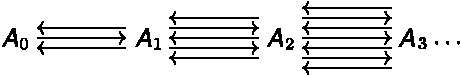
\includegraphics{simplicial_abgrp} \\
	met de 5 vergelijkingen
\end{center}

Ketencomplexen:
\begin{center}
	$ C_0 \from C_1 \from C_2 \from \cdots $ \\
	met $\del \circ \del = 0$
\end{center}

\pause $\sAb$ heeft meer structuur?
\end{frame}

\begin{frame}{De Dold-Kan correspondentie}
	$$ \visible<2->{N:} \sAb \only<1>{\simeq} \only<2->{\rightleftarrows} \Ch{\Ab} \visible<2->{:K} $$
	
	\visible<2->{
	\begin{align*}
		\text{Zodat}\qquad &\forall C \in \Ch{\Ab}: &N(K(C)) \iso C \\
		\text{en}\qquad &\forall A \in \sAb: &K(N(A)) \iso A.
	\end{align*}
	}

	\bigskip\visible<3->{
	$N$ is in zekere zin surjectief: $\forall C \in \Ch{\Ab}$ is er een $A \in \sAb$ met $N(A) \iso C$.
	}
\end{frame}

\begin{frame}{Eerste gok}
	Definieer $M: \sAb \to \Ch{\Ab}$ met $M(A)_n = A_n$.

	\bigskip\pause
	Zij $C = \Z \from 0 \from 0 \from \cdots$\\
	Is er een $A$ zodat $M(A) \iso C$?\\
	M.a.w. $A_0 \iso \Z$ en $A_1 \iso 0$, kan dat?

	\bigskip\pause
	Nee! Want $A_0 \tot{A(\sigma_0)} A_1$ is injectief!\\
	(want $\sigma_0 \delta_0 = \id$, dus $A(\delta_0)A(\sigma_0) = \id$)
\end{frame}

\begin{frame}{Definities}
	Zij $A \in \sAb$ \\
	$x \in A_n$ heet een \emph{$n$-simplex} \\
	$x \in A_n$ is \emph{gedegenereerd} als $x = A(\sigma_i)(y)$ voor een zekere $i$ en $y$.
\end{frame}

\begin{frame}{De juiste constructie}
	Zij $A \in \sAb$, definieer
	\begin{align*}
		N(A)_n &= \bigcap_{i=1}^n \ker(A(\delta_i)) \\
		\del &= A(\delta_0)
	\end{align*}
	\pause
	\begin{lemma}
		$x \in N(A)_n$ is niet-gedegenereerd.
	\end{lemma}
	\bigskip
	\begin{lemma}
		\centering$ A_n = N(A)_n \oplus D_n(A). $
	\end{lemma}
\end{frame}

\begin{frame}{Voorbeeld}
	Definieer de volgende simpliciaal abelse groep:
	\begin{gather*}
		A_n = \Z \\ 
		A(\delta_i) = A(\sigma_i) = \id.
	\end{gather*}

	\pause
	$$ N(A) = \Z \from 0 \from 0 \from \cdots. $$
\end{frame}

\begin{frame}
	\begin{center}
	$$ N: \sAb \rightleftarrows \Ch{\Ab} :K $$
	\pause\bigskip
	\Huge Vragen?
	\end{center}
\end{frame}


\end{document}
